\documentclass[12pt, a4paper,oneside]{book}
% Подключение библиотеки
\usepackage{/Users/vladbelousov/Desktop/Semestr_4-FP-NSU/Настройка/library}

\begin{document}

\begin{titlepage}
    \thispagestyle{empty}  % Отключаем нумерацию страницы на титульном листе
    \centering
    \vspace*{1cm}  % Отступ сверху

    \textbf{\huge Конспект лекций по дисциплине}  \\[1.5cm]  % Название
    \textbf{\huge Основы функционального анализа}  \\[2cm]   % Название дисциплины (оставьте пустым для добавления вручную)
    \textbf{\Large Новосибирский государственный университет} \\[0.5cm]
    \textbf{\large Физический факультет} \\[0.5cm]
    \textbf{\large 4-й семестр} \\[0.5cm]
    \textbf{\large 2025 год} \\[10cm]

    \begin{flushright}
        \large Студент: Б.В.О \\[0.5cm]  % Ваше имя
        Преподаватель: Ротанова Татьяна Александровна  % Ф.И.О. преподавателя
    \end{flushright}
\end{titlepage}

\tableofcontents  % Создание оглавления

\def\mainfile{}  % Определяем макрос для основного файла
% Условная компиляция для самостоятельной работы
\ifdefined\mainfile
    % Если это часть основного файла, не добавляем начало и конец документа
\else
    \documentclass[12pt, a4paper]{report}
    \usepackage{/Users/vladbelousov/Desktop/Semestr_4-FP-NSU/Настройка/library}
    \usepackage[utf8]{inputenc} % Подключение поддержки UTF-8
    \begin{document}
\fi

%%-------------------------------%%

\chapter{Геометрия пространств со скалярным произведением.}

\begin{center}
    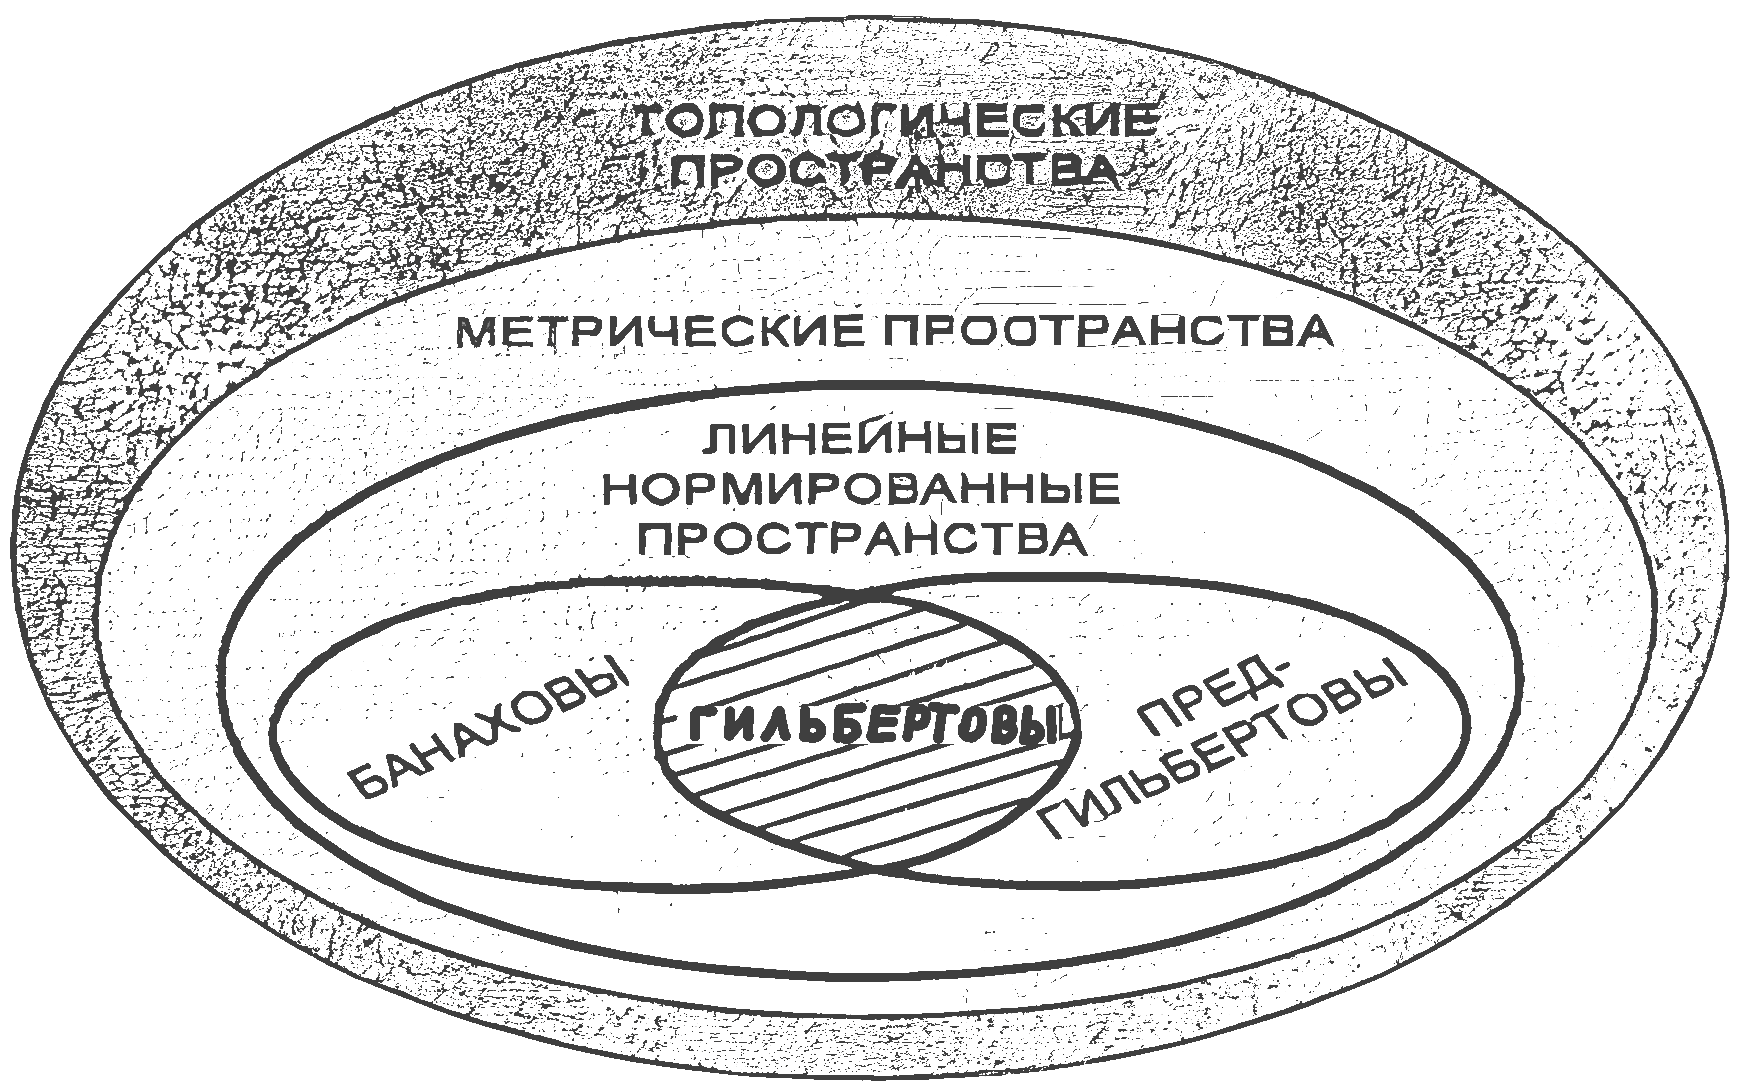
\includegraphics[width=0.5\textwidth]{/Users/vladbelousov/Desktop/Semestr_4-FP-NSU/ОФА/Лекции_по_дням/image/1.png}
\end{center}

\begin{definition}[Метрическое прострнвство]
    Метрика \( \rho (x,y): M ^2 \to  \mathbb{R} \) 

    1) \( \forall x,y :\rho (x,y ) \geq 0 - ( \rho(x,y) = 0 \Leftrightarrow x=y)   \) 

    2) \( \forall x,y \in  M :\rho(x,y )= \rho (y,x)  \)
    
    3) \( \forall x,y,z :\rho(x,z) \le  \rho(x,y)+\rho(y,z) \)
\end{definition}

\( B_{\varepsilon}(x) = \{ y \in  M | \rho(x,y) < \varepsilon \} \) 

\begin{definition}
    Множество открытое, если любая точка в нем содержится в нем вместе некоторой окрестностью.
\end{definition}

Пример дискреткой метрики: 

\[ 
\rho(x,y) = 
\begin{cases} 
    1 \quad x \neq y \\
    0 \quad  x=y   
\end{cases} 
\] 

\section{Линейно (векторное) пространство}

\begin{definition}
    Непустое множество элементов L произвольной природы, называется линейным (векторным) над полем чисел \( \mathbb{R} (\mathbb{C})\) если 

    1) \( \forall x,y   \) введена операция сложения:

    \( \quad  \) 1.1)  \( x+y = y+x \) (коммутативность)
    
    \( \quad  \) 1.2) \( x+(y+z)= (x+y ) +z \) (ассоциативность)
    
    \( \quad  \) 1.3) В L существует элемент называемым нулем 0: \( x+0 = x \text{ }  , \forall x \in  L \)  

    \( \quad  \) 1.4) \( \forall x \in  L \)  существует противоположный элемент принадлежащий 
    
    L: \( x+y = 0 \) , обозначается как \( -x \)

    2) \( \forall x \in  L \)  и \( \forall  \) числа \( \alpha \in  \mathbb{R}(\mathbb{C}) \) определен вектор из L - произведения элементов на число \( \alpha , \alpha x \in  L \):
    
    \( \quad  \) 1.1) \( \alpha (\beta x )= (\alpha \beta )x  , \forall  \alpha, \beta  \)
    
    \( \quad  \) 1.2) \( 1 \cdot x =x  \) (существования единицы)
    
    \( \quad  \) 1.3) \( \alpha (x+y) = \alpha x + \alpha y \)

    \( \quad  \) 1.4) \( (\alpha + \beta )x = \alpha x + \beta x \) 


\end{definition}

Примеры: 

1)
\[ \begin{aligned}
\begin{array}{ll}
    \mathbb{R}^{n }\\
    \mathbb{C}^{n}  
\end{array}
\begin{array}{ll}
    \quad \alpha(x_1,x_2, \ldots, x_n) \\
    + \\
    \quad \beta (y_1,y_2, \ldots ,y_n )
\end{array}
\quad =(\alpha x_1 + \beta y_1 ,\dots \alpha x_n + \beta y_n)
\end{aligned} \] 

2) \( C[a,b] = \{f(a,b) \to  \mathbb{C}, \text{ непрерывная функции } f \text{ - непрерывна }   \)\}

3) \(\displaystyle  L_p (x)= \{f \text{- измерима по Лебегу, заданная на } X , f: X \to  \mathbb{C} \text{ таких, что }   \)

\[  \int_{X}|f(x)|dx< \infty  \] 

4) \(\displaystyle  l_2 : x = \{x_1 , \ldots , x_n  \} \quad \sum ^{\infty }_{1}  |x_n| ^2 < \infty  \) 

\begin{definition}
    \( x_1, \ldots, x_n \)  называется линейно зависимыми, если \( \exists \alpha_1 , \ldots , \alpha _ n   \) не все равные нулю, такие что \( \alpha_1 x_1 + \dots + \alpha_n x_n=0   \)
    
    В противном случае: из того, что \( \alpha_1 x_1 + \dots + \alpha_n x_n=0 \) следует, что все \( \alpha_i =0  \) \( x_1, \ldots, x_n \)  называется линейно независимыми наборами  векторов.  
\end{definition}

\begin{definition}
    Бесконечный набор элементов L называется линейно независимым, если любой его конечный поднабор линейно независимым.
\end{definition}

\begin{definition}
    Если в L можно найти \( n  \)  линейно независимых векторов, а любой набор из \( n+1 \) векторов является линейно зависимыми, то \( \dim L= n \). Если в L можно указать   набор из произвольного числа линейно независимых элементов, то \( \dim L= \infty  \). 
\end{definition}

\begin{definition}
    Непустое подмножество \( S \subset L  \)  называется подпространством, если оно само является пространством введенных в L линейных операций.
\end{definition}

\begin{definition}
    Линейной  оболочкой  <M> называется совокупность всех линейных комбинаций  \( \alpha x + \beta y  \)  где \(  x,y \in  M  \subset \alpha, \beta \in  \mathbb{C}(\mathbb{R}) \) 

    <M> - подпространство в L  (натянутое или порожденное множеством элементов M)
\end{definition}


\begin{definition}
    Норма в линейном пространстве L:  \( \norm{\text{ } }  : L \to  \mathbb{R}^+ = [ 0 , \infty ) \)

    \( \forall x,y \in  L ,  \forall  \alpha \in  \mathbb{C}(\mathbb{R}) \) 
    
    1) \( ||x|| \geq  0 ,||x||=0 \Leftrightarrow x=0  \quad   \) (положительная определенность нормы)
    
    2) \( ||\alpha x||=|\alpha|||x || \quad  \)  (положительная однородность нормы) 

    3) \( ||x+y|| \le  ||x|+||y|| \)
\end{definition}

В конечномерных пространствах все нормы эквиваленты \( c_1||x||_1 \le  ||x||_2 \le  c_2 ||x||_1 \). В конечномерных пространствах это не так! 

Пример норм: 

\[1)  \norm{f}= \max _{t \in [ a,b]} |f(t)| \text{ - норма в }  C [ a,b]  \text{ равномерная норма.}  \] 

\[ \begin{aligned}
    2) &  \quad ||f||_{L_1} = \int_{X} |f|dx \text{ в  }  L_1 \\
    3) & \quad ||f||_{L_p} = \sqrt[p]{\int_{X}|f|^p dx} \text{в}  L_{p} \\
    4) & \quad ||x||_{l_2}= \sqrt{\sum^{\infty }_{i=1} |x_i| ^2   }   
\end{aligned} \] 

\begin{definition}
    Последовательность \( (x_n)_{n \in  N}  \) точек линейно нормированное пространств L сходятся к x, если  \( ||x_n - x|| \xrightarrow{n \to  \infty } 0 ,\forall \varepsilon > 0, \exists n_0, n > n_0 : ||x_n - x|| < \varepsilon   \) 
\end{definition}

\begin{definition}
    Предельной точкой \( M \subset L  \)  называется точка x, если существует сходящаяся к x последовательность элементов из M \( \exists x_n \in  M : x_n \to x  \) 
\end{definition}

\begin{definition}
    Замыканием \( \overline{M}  \) - объединение  M и его предельных точек (по конкретной норме). 
\end{definition}

\begin{definition}
    Множество замкнутое, если содержит все предельные точки.
\end{definition}

\begin{definition}
    Множество M в L - линейно нормированном пространстве называется плотным в L, если \( \overline{M}= L  \) 
\end{definition}

\begin{definition}
    Сепарабельное множество, если в нем \( \exists  \) счетное плотное подмножество
\end{definition}



%%-------------------------------%%

% Закрытие документа, если файл компилируется отдельно
\ifdefined\mainfile
    % Если это основной файл, не нужно заканчивать документ
\else
    \end{document}
\fi
% Условная компиляция для самостоятельной работы
\ifdefined\mainfile
    % Если это часть основного файла, не добавляем начало и конец документа
\else
    \documentclass[12pt, a4paper]{report}
    \usepackage{/Users/vladbelousov/Desktop/Semestr_4-FP-NSU/Настройка/library}
    \usepackage[utf8]{inputenc} % Подключение поддержки UTF-8
    \begin{document}
\fi

%%-------------------------------%%

Пример: Множество множеств P[0,1] не является замкнутым подпространством в C[0,1]

\[ P_n (x )  \to  f(x ) \Leftrightarrow  \left\lVert P_n - f  \right\rVert _C \to  0 \]

\[ \forall  n , p_n \in  P[0,1] , f(x ) \in  C[0,1] - \text{не является полиномом} \] 

\[ p_n(x) = 1+ x + \frac{x ^2 }{2 }  + \dots + \frac{x^n }{n!}  \] 

\[  f(x ) = e ^{x} , \quad f(x ) = f(0 ) +\frac{f'(0)}{1!}x+\frac{f''(0 )}{2!}x^2+\dots+ \frac{f^{(n )(0)} }{n ! }x^{n } + \frac{f^{(n+1 )(c)} }{(n+1)!} x^{n+1}     \] 

Замыкание \( P[0,1] \)  это \( L_2[0,1] \) 

\[ \left\lVert p_n -f  \right\rVert _{L_2}  \le  \max_{x \in [0,1]} \max_{c \in  [0,1]} \left\lvert \frac{e^c x^{n+1 } }{(n+1)!}  \right\rvert  \overset{\tiny\begin{aligned} x=1 \\c=1\end{aligned}}{=}\frac{e}{(n+1)!} \xrightarrow{n \to  \infty } 0 ,\quad e^x \notin P[0,1]       \] 



\[ L_2 (x ) :\{f: X \to  Y , \int_{x} |f| ^2 dx < \infty \} \] 

\[ \left\lVert f  \right\rVert _{L_2 } = \sqrt{\int_{x }|f| ^2 dx} \] 

Нуль: \( f : X \to  Y  \) 

\[  0(x ) : X \to  Y \] 

\[ g=0(x ) = 0 - \text{почти всюду}  \] 

\[ g = \begin{cases}
    0 , \mathbb{R}  /\mathbb{Q} \\
    \infty , \mathbb{Q}  
\end{cases} \] 


Элементы (вектора) пространства \( L_2    \)  - функции класса \( L_2  \) .

\begin{definition}
    Последовательность \( (x_n )_{n \in  \mathbb{N}} , x_n \in  L \) (линейно нормированное пространство) называется фундаментальной, если \( \forall  \varepsilon >0 , \exists N , \forall m,n >N : \left\lVert x_m - x_n  \right\rVert < \varepsilon \) 
\end{definition}

\begin{definition}
    Если любая фундаментальная последовательность является сходящейся в L, то L - полное пространство.
\end{definition}

\begin{definition}
    Полное нормированное пространство - банахово пространство
\end{definition}

\section{Линейные пространства с скалярным произведением}

\begin{definition}
    Скалярное произведение в L (, ) : \( L \times L \to  \mathbb{C} \). \( \forall x_1,x_2, y \in  L, \alpha_1,\alpha_2 \in \mathbb{C}(\mathbb{R}) \) выполняется: 

    1) \( (\alpha_1 x_1 + \alpha_2 x_2, y ) = \alpha_1(x_1,y )+ \alpha_2 (x_2,y) \) 

    2) \( (x,y ) = (\overline{y,x} )\)  

    3) \( (x,x ) \ge  0 \quad \text{и}  \quad  (x,x ) = 0 \Leftrightarrow x =0\) 
\end{definition}

Линейное пространство со скалярным произведением над \( \mathbb{R}   \) - евклидовы пространства, над \( \mathbb{C}    \) - унитарное пространства. 

\[ 1) \mathbb{R} ^ n ( \mathbb{C}^ n ): (x, y ) = \sum  ^{n }  x_i \overline{y } _i   \] 

\[ 2) l_2 : (x,y ) = \sum ^{\infty  } x_i \overline{y } _i   \] 

\[ 3) L_2(x ) : (f,g )= \int  _{x } f \overline{g } dx   \] 

\[ 4) C[a,b ] : \text{ нет скалярного произведения согласованного  с аксиомами нормы} \] 

\begin{lemma}
    Величина \( \left\lVert x  \right\rVert = \sqrt{(x,x)} \) удовлетворяет свойствам нормы. Согласованная или порожденная скалярным произведением.
\end{lemma}


\begin{definition}
    Гильбертово пространство - пространство со скалярным произведением, полное относительно нормы, порожденным этим скалярным произведением.
\end{definition}

\begin{lemma}[ Неравенство Коши-Буняковского]
    \( \forall x \in  L \quad  |(x, y )| \le  \left\lVert x  \right\rVert \left\lVert y \right\rVert \) 
\end{lemma}

\begin{proof}
    \[ \alpha = \frac{(x,y )}{|(x,y )|} , \quad  t \in  \mathbb{R} \] 

    \[ 0 \le  \left\lVert \overline{\alpha} x +  ty \right\rVert ^2 = ( \overline{\alpha } x+ ty , \overline{\alpha } x + ty     ) = \overline{\alpha }( x, \overline{\alpha }x _ty  ) + t(y , \overline{\alpha }x + ty  )=   \] 

    \[  \underbrace{|\alpha | ^2}_{=1} ( x,x ) + \overline{\alpha } t ( x,y ) + \alpha t ( y ,x ) + t ^2 ( y,y )=  \left\lVert x  \right\rVert ^2 + \overline{\alpha } t (x, y ) + \alpha t ( y ,x ) + t ^2 \left\lVert  y  \right\rVert ^2 \boxed{=}    \] 

    \[\overline{\alpha }t (x,y )+ \alpha t ( y ,x )  =t  \left( \frac{(\overline{x,y }  ) ( x,y)}{|(x,y)|}+ \frac{({x,y }  ) (x,y)}{|(x,y)|} \right)  = 2t |(x,y)|\] 

    \[ \boxed{=} \left\lVert x   \right\rVert  ^2 + 2t |(x,y)   |+ t ^2 \left\lVert y  \right\rVert ^2\] 

    \[ |(x, y )| \le  \left\lVert x  \right\rVert \left\lVert y \right\rVert \] 
\end{proof}

\begin{proof} [Доказательство Леммы 1]

    1) Из 3 аксиомы скалярного произведения; 

    2) \( \alpha \in  \mathbb{C}, \left\lVert \alpha x    \right\rVert ^2 = |\alpha | ^2 \left\lVert x  \right\rVert ^2 =(1) \)
    
    \[ (\alpha x , \alpha x ) = \alpha ( x, \alpha x ) = \alpha \overline{\alpha } ( x,x)  = (1 ) \] 

    3) \( \left\lVert x + y  \right\rVert \le  \left\lVert x  \right\rVert \left\lVert y \right\rVert \) 

    \[ \left\lVert  x+ y  \right\rVert ^2 = ( x+ y , x+ y )  = ( x, x+ y ) + ( y , x+ y ) = ( \overline{x+ y , x }  ) + ( \overline{x+ y , y }  ) = (\overline{x,x }   ) + ( \overline{y,x }   )  +( \overline{x, y }  ) + ( \overline{y, y }  ) = \] 

    \[ = \left\lVert  x  \right\rVert  ^2 +  (x, y ) + (y,x ) +  \left\lVert y  \right\rVert ^2 \le  \left\lVert x  \right\rVert ^2 + 2 |(x,y)   | + \left\lVert y  \right\rVert ^2  \le  \] 

    \[ \overset{\text{нер-во К-Б} }{\le}  \left\lVert x  \right\rVert ^2 + 2 \left\lVert x  \right\rVert \left\lVert y  \right\rVert+ \left\lVert y  \right\rVert ^2 = ( \left\lVert  x  \right\rVert + \left\lVert  y  \right\rVert) ^2  \] 
\end{proof}


\[ L_2 : \sqrt{ \int  _x |f(x)| ^2 dx    } = \left\lVert f  \right\rVert _{L_2}  \] 

\[ \left\lvert \int_{x }  f (x ) \overline{g }  (x ) dx        \right\rvert  \le  \left( \int_{x }|f(x ) | ^2 \right) ^{\frac{1}{2 } } \left( \int_{x } |g(x)| ^2 dx   \right) ^{\frac{1}{2} } - \text{ неравенство К-Б в }  L_2     \] 

\[ \sqrt[  p ]{\int_{x }|f(p)|dx}= \left\lVert f  \right\rVert _{L_p} \]  

\begin{lemma}
    \( \forall p \geq 1   \) линейно нормированное пространство  \( L_ p   \)  является полным.  
\end{lemma}

\begin{lemma}
    \( \forall  p \geq 1   \)  пространство \( C^{\infty }  \) плотно в \( L_p (x) \), то есть \( \overline{C}^{\infty ^{L_p} }= L_p(x)    \)   
\end{lemma}

\begin{lemma}
    \( \forall  p \ge 1  \)  пространство \( L _ p  \)  сепарабельно.
\end{lemma}

\begin{lemma}
    Пусть L - линейно нормированное пространство со скалярным произведением и норма порождена скалярным произведением\dots

    \[ \forall  x, y \in  L \quad  \left\lVert x+ y  \right\rVert ^2 + \left\lVert  x- y  \right\rVert ^2 = 2 (\left\lVert x   \right\rVert ^2 + \left\lVert y  \right\rVert ^2) - \text{равенство паралеллограма} \] 
\end{lemma}

Наоборот, если в линейно нормированном пространстве L выполняется равенство паралеллограма, то в этом пространстве можно ввести скалярное произведение, согласованной с этой нормой.

\( L_1 \subset [ a, b ] \exists  f,g ,   \)  для которых не выполняется равенство паралеллограма \( \Rightarrow      \) нельзя ввести скалярное произведение, согласованное с нормой.

\begin{lemma}
    В линейном  пространстве со скалярным произведением  L , скалярное произведение непрерывно по первому аргументу относительно сходимости по норме порожденной скалярным произведением

    \[ x_n \to  t \quad \left\lVert x_n - x           \right\rVert  \xrightarrow{n \to  \infty }  0  \] 

    \[ \forall y , (x_n, y  ) \to  (x, y ) \] 
\end{lemma}

\begin{proof}

    \[ |(x_n, y ) -(x,y )  | = |(x_n- x,y ) | \overset{\text{по К.Б} }{\le}  \left\lVert x_n - x  \right\rVert \underbrace{\left\lVert y \right\rVert}_{\text{огр.числено} } \xrightarrow{x \to  \infty } 0   \] 
\end{proof}

\section{Ортогональность векторов}

\begin{definition}
    L  - пространство со скалярным произведением, \( x, y \in  L \) называется ортогональным, если \( (x,y ) = 0   \) 

    
\end{definition}

\begin{definition}
    Набор векторов \( x, \ldots, x_n, \ldots,   \in  L \) называется ортогональным, если \( \forall  ij : x_i \perp x_j  \) 
\end{definition}


\begin{definition}
    Набор ортогональный ( \( x_n     \) ) называется ортнармированным, если \( \forall  i :  \left\lVert x  \right\rVert = 1   \) 
\end{definition}

Ортогонализация Грамма-Шмидта

Если \( x_1, \ldots, x_n  \)  - счетная система линейно назависимый в  L , тогда новые последовательности: 

\[ y_1 = x_1 \quad  z_1 = \frac{y_1}{\left\lVert y_1  \right\rVert}  \] 

\[ y_2 = x_2 - ( x_2 , z_1 ) z_1  \quad  z_2 = \frac{y_2}{\left\lVert y_2  \right\rVert} \] 

\[ y_n = x_n - \sum ^{n-1 }_{k =1}( x_n , z_k ) z_k  \quad  z_n = \frac{y_n}{\left\lVert y_n  \right\rVert}    \] 

Обладает свойствами: 

1) Система \( z_1, \ldots, z_n   \) - ортонормированна

2) \( \forall n \in  N \underset{\text{линейные оболочки } }{\underbrace{<z_1, \ldots, z_n >} = \underbrace{<x_1, \ldots, x_n>}}\) 
%%-------------------------------%%

% Закрытие документа, если файл компилируется отдельно
\ifdefined\mainfile
    % Если это основной файл, не нужно заканчивать документ
\else
    \end{document}
\fi
% Условная компиляция для самостоятельной работы
\ifdefined\mainfile
% Если это часть основного файла, не добавляем начало и конец документа
\else
\documentclass[12pt, a4paper]{report}
\usepackage{/Users/vladbelousov/Desktop/Semestr_4-FP-NSU/Настройка/library}
\usepackage[utf8]{inputenc} % Подключение поддержки UTF-8
\begin{document}
\fi

%%-------------------------------%%

\begin{definition}
     Углом между ненулевыми векторами x и y  евклидова пространства \( L  \)  называется число \( \varphi \in  [ 0, \pi ] \):

     \[ \cos \varphi = \frac{(x,y )}{\left\lVert x  \right\rVert \left\lVert y  \right\rVert}  \] 
\end{definition}

\begin{definition}
    Если S - подпространство пространства со скалярным произведением \( L \), то \( x \in  S  \)  называется вектором наилучшего приближения (ближайший) для \( y \in L      \)  посредством векторов из \( S  \), если: 

    \begin{center}
        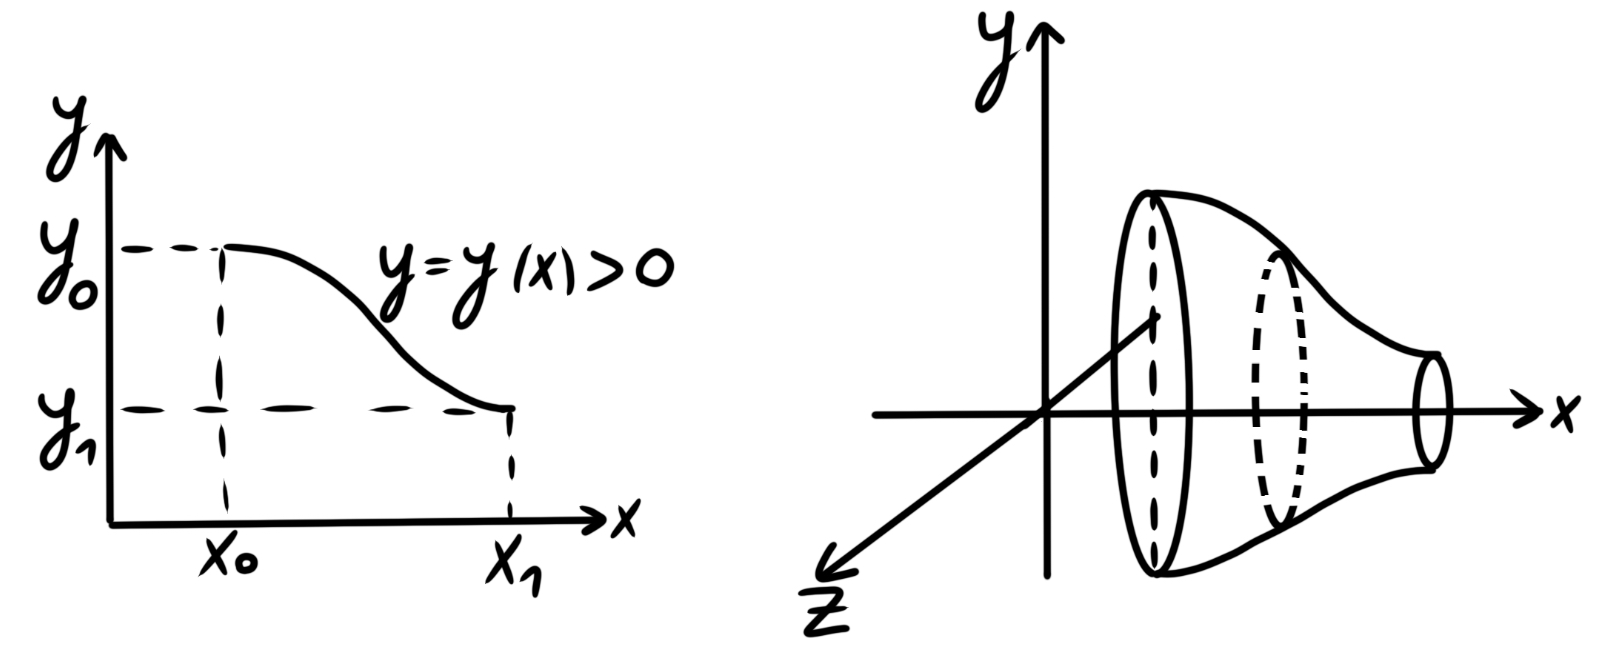
\includegraphics[width=0.3\textwidth]{/Users/vladbelousov/Desktop/Semestr_4-FP-NSU/ОФА/Лекции_по_дням/image/2.png}
    \end{center}

    \[ \forall z \in  S , \quad  \left\lVert y - z  \right\rVert \geq  \left\lVert x - y  \right\rVert \] 

    \[ \left\lVert x - y  \right\rVert  = \inf _{z \in  S } \left\lVert y -z  \right\rVert  \] 
\end{definition}

\begin{theorem}
    Пусть \( H  \)   - гильбертово пространство, \( S  \)   - замкнутое подпространство \( H , \text{  }  y \in  H  \), тогда \( \exists  ! x  \) ближайший к y.
\end{theorem}

\begin{proof}

    \[ \inf \left\lVert y -z  \right\rVert = d  \]  

    \[ x_1, \ldots, x_m \in  S \quad  \left\lVert  y - x_m       \right\rVert \xrightarrow{m \to  \infty } d   \] 

    \[ \left\lVert x_m - x_n         \right\rVert ^2 = \left\lVert (x_m - y ) - (x_n - y )  \right\rVert  ^2 = 2( \left\lVert  x_m - y   \right\rVert ^2 + \left\lVert  x_n - y      \right\rVert ^2 ) - \underset{_{\left\lVert x_m+ x_n - 2y  \right\rVert ^2 = 4 \left\lVert q - y  \right\rVert ^2 \geq 4 d ^2  }}{\left\lVert \underbrace{x_m - y + x_n - y }  \right\rVert }^2 \boxed{\le } \] 

    \[ q = \frac{x_m+ x_n }{2 } \in  S   \] 

    \[  \forall  \varepsilon , \exists  N \text{ }  n, m \geq  N :  \left\lVert x_m - y      \right\rVert  < d ^2 + \varepsilon \quad  \left\lVert  x_n - y  \right\rVert  ^2 \le  d ^2 + \varepsilon \] 

    \[ \boxed{\le  } 4 d ^2 + 2 \varepsilon - 4 d ^2 = 2 \varepsilon   \] 

    \[ x_m - \text{ фундаментальная }  \] 

    \[ \text{существование предела последовательности }   x: \] 

    \[  x \in  S , \text{ т.к }  S - \text{ замкнутое}  \] 

    \[ \left\lVert  y - x_n      \right\rVert = \sqrt{(y - x_n , y - x_n )} \underset{(1)}{\xrightarrow{n \to  \infty  } }\sqrt{(y - x, y -x )} = \left\lVert y -x  \right\rVert \to  d \text{ в силу ! предела}    \] 

    \begin{center}
        (1) - непрерывность по 1-му аргументу
    \end{center}

    Единственность: 

    \[ \text{Пусть } \tilde{x }: \left\lVert  y - \tilde{ x }\right\rVert = d , x \neq  \tilde{x } \] 

    \[ \left\lVert  \tilde{ x } - x      \right\rVert ^2 = \left\lVert  (\tilde{x }- y ) - ( x - y ) \right\rVert ^2 = 2\underset{= d ^2 }{\left\lVert \underbrace{\tilde{x }  - y}  \right\rVert}  ^2 +2\underset{= d ^2 }{\left\lVert \underbrace{x  - y}  \right\rVert} ^2 - \left\lVert 2 y - x - \tilde{x } \right\rVert ^2 \le 4 d ^2 - 4 d ^2 \le  0 \] 

    \[ \text{т.е } \tilde{x } = x - \text{ противоречие }  \] 

\end{proof}

\begin{definition}
    \( S  \)  - подпространство в линейном пространстве со скалярным произведением \( L, \text{ } x \in  S   \)  - ортогональная проекция \(  y \in  L   \)  на подпространство \( S  \), если: 

    \[ y- x \perp  S \quad  y -x \perp  z \text{ }  \forall  z \in  S \quad  ( y - x , z ) = 0  \] 

\end{definition}


\begin{lemma}
    \( S  \)  - подпространство в линейном пространстве со скалярным произведением \( L, \text{ }  x \in  S  \)  - ортогональная проекция \(  y \in  L  \Leftrightarrow   \)   x - ближайший к y посредством S.
\end{lemma}

\begin{proof}

    \[  \] 

    \( \boxed{\Rightarrow} :\) 
    
    \[ \forall  x, y , z \in  L \] 

    \[ \left\lVert  y - z  \right\rVert ^2  = ((y -x )+ (x- z ), (y -x) + ( x - z)) =   \] 
    
    \[ \overset{(1)}{=} \left\lVert y -x    \right\rVert ^2 + 2 \mathrm{Re }( \cancelto{0 }{x- y , x -z }) + \left\lVert x -z  \right\rVert ^2 (* ) \] 

    \[ (1): (a+b, a+ b )   = \left\lVert  a  \right\rVert ^2 + \left\lVert  b  \right\rVert ^2 + 2 \mathrm{Re } ( a,b ) \] 

    \[ x \in  S - \text{ ортогональная проекция y  на }  S \Rightarrow y -x \perp  x-z   \]  

    Итого: 

    \[ \left\lVert  y -z  \right\rVert ^2 = \left\lVert  y -x  \right\rVert ^2 + \underset{\geq 0 }{\left\lVert \underbrace{ x- z}  \right\rVert }^2  \] 

    \[ \forall  z \in  S : \left\lVert  y -z  \right\rVert ^2 \le  \left\lVert  y -x  \right\rVert ^2 , x - \text{ ближе для y }  \] 

    Пусть дано: 

    \( \boxed{\Leftarrow}: \) 

    \[ x - \text{ ближайший вектор для  } y \in S   \] 





    \[ \begin{aligned}
        \begin{array}{l|}
            \left\lvert y -x  \right\rvert = \inf \left\lVert  y -z \right\rVert \\
            f(t )  = \left\lVert  y -x + t W  \right\rVert ^2, \quad  t \in  \mathbb{R}  ^2 , \text{ }  W \in S
        \end{array}
        \Rightarrow f' (0 ) =0 
    \end{aligned} \] 

    \[ \lim_{t  \to 0}  \frac{ \left\lVert y -x + t W  \right\rVert ^2 - \left\lVert  y -x  \right\rVert ^2 } {t } = 0   \] 

    \[ \text{ в } (* ): z = x - t W  \]
    
    \[ \left\lVert y - (x - tW ) \right\rVert  ^2 - \left\lvert y -x  \right\rvert  ^2 = 2 \mathrm{Re } (y - x, t W ) + \left\lVert t W  \right\rVert ^2   \] 

    \[ \lim_{t  \to 0}    t\frac{2 \mathrm{Re } (y - x , W ) }{ t } + t ^2         \cancelto{0 }{ \frac{\left\lVert W  \right\rVert ^2 }{t } } = 0      \] 

    \[ 2 \mathrm{Re }  ( y - x, W )  = 0  \] 

    Если \( \mathrm{Im } ( y -x , W ) = 0 \), то x - ортогональная проекция y на S.

    Доказывается аналогично: \( f(t ) = \left\lVert y -x + i t W \right\rVert ^2 \)  

\end{proof}

\begin{definition}
    S - подпространство линейного пространства L  со скалярным произведением, то совокупность всех \( x \in  L    \), таких, что \( x \perp y \text{ }  \forall  y \in S  \) называется ортогональным дополнением к S  (\( S^{\perp }  \)).
\end{definition}

\begin{definition}
    Линейное пространство L является прямой суммой S  и T если любой вектор \( x \in  L      \)  единственным образом представим в виде \( x = y + z , \text{ }  y \in  S , \text{  } z \in  T  \) 
\end{definition}

\begin{lemma}
    H - гильбертово пространство, S - замкнутое подпространство, тогда H  прямая сумма S  и \(  S^{\perp } \) , \( H =   S \oplus S^{\perp }   \) 
\end{lemma}

\begin{proof}
    
    \[  y \in  H \quad  x - \text{ ближайший к y посредством S } \Rightarrow  \] 

    \[ \overset{\text{Лемма 1} }{\Rightarrow} y -x \perp  z , \text{ }  z \in  S \Rightarrow  \] 

    \[\Rightarrow  W = y -x \in  S^{\perp }  \]  

    \[ y = \overset{ \in  S ^{\perp } }{W} +\overset{\in  S }{ x}  \] 

    Докажем единственность представления: 

    Пусть \( y = \overset{ \in  S ^{\perp } }{\tilde{W }} + \overset{ \in  S ^{\perp } }{\tilde{ x }}  \) 

    \[  W + x = \tilde{ W } +\tilde{ x } \] 

    \[ W - \tilde{W } = \tilde{ x } - x  \] 

    \[ (\underset{\in  S ^{\perp }}{W- \tilde{W }}  , \underset{\in S}{ \tilde{ x } - x }) = (\tilde{x } -x , \tilde{x } - x ) \] 

    \[ 0 =  (\tilde{x } -x , \tilde{x } - x )\] 

    То есть: \( \tilde{x } = x  \text{ и }  \tilde{W } = W  \) 
\end{proof}

\begin{theorem}
    S - конечномерное подпространство линейного пространства L со скалярным произведением \( x_1, \ldots, x_n    \)  - ортонормированный базис в S\( \forall  y \in  L     \):

    \[ x = \sum_{1} ^n \lambda_k x_k , \quad  \lambda_k = (y , x_k) \] 

    является ортогональной проекцией y на подпространство S. При этом: 

    \[  \left\lVert  y  \right\rVert ^2 =\left\lVert  x  \right\rVert ^2 + \left\lVert  y -x   \right\rVert ^2  \] 
\end{theorem}


\begin{proof}
    \[ \forall  z \in  S , \text{ }  z = \sum_{1} ^ n \alpha_k x_k  \] 

    \[  (z, x_m ) = \sum  _1 ^1 \alpha_k (x_k , x_m ) = \alpha_m \] 

    \[ \left\lVert z  \right\rVert ^2 = \left(  \sum  _ 1 ^ n \alpha_k x_k ,  \sum  _ 1 ^ n \alpha_p x_p  \right)  = \sum  _ 1 ^ n \alpha_p \left( \overline{\sum_1 ^ n \alpha_k x_k , x_p  }  \right) =\sum  _1 ^ n \alpha_p \left[ \sum  _1 ^ n \overline{\alpha_k } (\overline{x_p, x_k}  )   \right] =  \sum  _{k =1 }  ^{ n} \left\lvert  \alpha_k     \right\rvert  ^2 \]  

    \[ \left\lVert y -z  \right\rVert ^2 = \left\lVert y   \right\rVert ^2 - ( z, y ) -  ( y , z ) + \left\lVert z   \right\rVert ^2 = \left\lVert y  \right\rVert ^2 - \sum   _ 1 ^ n \alpha_k(x_k, y ) - \sum_{ 1} ^ n \overline{\alpha_k} (y, x_k ) +\sum_{ 1} ^n \left\lvert \alpha_k   \right\rvert ^2  = \]

    \[ =\left\lVert y  \right\rVert ^2 - \sum_{ 1 } ^ n \alpha_k \lambda_k - \sum_{ 1 } ^ n \overline{\alpha_k }\lambda_k +\sum_{ 1 } ^ n \left\lvert \alpha_k   \right\rvert ^2 +  \sum_{ 1 } ^ n \left\lvert \lambda_k      \right\rvert ^2- \sum_{ 1 } ^ n \left\lvert \lambda_k      \right\rvert ^2 = \left\lVert  y  \right\rVert ^2 + \sum_{ 1 } ^ n \left\lvert  \alpha_k - \lambda_k \right\rvert ^2  -\sum_{ 1 } ^ n \left\lvert \lambda_k     \right\rvert ^2       \] 

    \[ \left\lVert y  \right\rVert ^2 - \sum_{ 1 } ^ n \left\lvert \lambda_k     \right\rvert ^2 \geq 0  , \text{ при }  \alpha_k = \lambda_k \text{ } (z = x )  \] 

    При z = x  достигается минимум \( \Rightarrow   \)  ортогональная проекция.

\end{proof}

\begin{definition}
    \( x_1, \ldots, x_n, \ldots,  \)  - ортонормированная система в линейном пространстве со скалярным пространством L: 

    \[ x \in  L \quad  \lambda_k = ( x , x_k ) - \text{ коэффициент Фурье x.}  \] 

    \[ \sum_{ n= 1 } ^{\infty } \lambda_k x_k - \text{ ряд Фурье расходится}  \] 


\end{definition}

\begin{theorem}[неравенстов Бесселя]    
    \( x \in  L  \)  - линейное пространство со скалярным произведением, \( \lambda_k  \)  - коэффициент Фурье, тогда:

    \[ \sum_{k =1}^{\infty  } \left\lvert  \lambda_k     \right\rvert ^2 \le  \left\lVert x  \right\rVert ^2  \] 


\end{theorem}

\begin{proof}
    \[ <x_1, \ldots, x_n> \] 

    \[ S_n = \sum_{k =1}^{n  }   \lambda_k x_k\] 

    \[\underbrace{ \left\lVert x - S_n   \right\rVert}_{> 0} ^2   + \left\lVert S_n      \right\rVert ^2 = \left\lVert x  \right\rVert ^2 \] 

    \[ \left\lVert  S_n      \right\rVert  ^2 \le  \left\lVert x  \right\rVert ^2 \] 

    \[ \left( \sum_{k=1} ^{n  } \lambda_k x_k , \sum_{k=1} ^{n  } \lambda_k x_k  \right) \le  \left\lVert x  \right\rVert ^2 \] 

    \[ \sum_{k=1} ^{n  } \left\lvert \lambda_k     \right\rvert ^2 \le  \left\lVert x  \right\rVert ^2 \] 

    \[ \sum_{k=1} ^{n  } \left\lvert \lambda_k     \right\rvert ^2 \le  \left\lVert x  \right\rVert ^2 \] 
    \[ \overset{\displaystyle \downarrow }{\text{ в пределе}}  \]

    \[ \sum_{k=1} ^{\infty  } \left\lvert \lambda_k     \right\rvert ^2 \le  \left\lVert x  \right\rVert ^2   - \text{ равенство Парсеваля}  \] 

\end{proof}



%%-------------------------------%%

% Закрытие документа, если файл компилируется отдельно
\ifdefined\mainfile
% Если это основной файл, не нужно заканчивать документ
\else
\end{document}
\fi
% Условная компиляция для самостоятельной работы
\ifdefined\mainfile
% Если это часть основного файла, не добавляем начало и конец документа
\else
\documentclass[12pt, a4paper]{report}
\usepackage{/Users/vladbelousov/Desktop/Semestr_4-FP-NSU/Настройка/library}
\usepackage[utf8]{inputenc} % Подключение поддержки UTF-8
\begin{document}
\fi

%%-------------------------------%%

\textbf{Коэффициенты Фурье: } \( x_1, \ldots, x_n \)  , \text{ } \( \lambda_k = (x, x_k) \)

\textbf{Неравенство Бесселя:} \( \displaystyle \sum_{k=1} ^{\infty } \left\lvert \lambda_k \right\rvert  ^2 \le  \left\lVert x \right\rVert ^2\) 

\section{Пополнение ортонормированной системы}

\begin{definition}
    Ортонормированную систему \( x_1, \ldots, x_n \) называют замкнутой, если для \( \forall  x \in  H  \): 

    \[ \left\lVert x  \right\rVert  ^2 = \sum _{k=1} ^{n  } \left\lvert \lambda_k     \right\rvert ^2 , \text{ где } \lambda_k = (x, x_k) - \text{ коэффициенты Фурье}   \] 
\end{definition}

Уравнение замкнутости:

\[  y \in  H , \mu_k = (y, x_k) - \text{ коэффициенты Фурье } y \] 

\[ (x,y ) = \left( \sum_{k=1} ^{\infty } \lambda_k x_k , \sum_{k=1} ^{\infty } \mu_k x_k  \right) = \sum _{k=1} ^{\infty } \lambda_k \overline{\mu_k }    - \text{ равенство Парсеваля} \] 

\begin{definition}
    Ортонормированная системам \( x_1, \ldots, x_n \) называется полной, если ее нельзя пополнить, то есть если ее ортогональное дополнение состоит только из \( \vec{0}  \). Другими словами, если \( \exists  x \text{ }  \forall  k : (x, x_k ) = 0 \Rightarrow x = 0 \)\dots

\end{definition}

\begin{definition}
    Ортонормированная система \( x_1, \ldots, x_n \) называется базисом Гильбертова (или Гильбертовым базисом), если \( \forall  x \in  H \):

    \[\underset{\text{разложение в векторный ряд Фурье} }{ x = \sum _{k=1} ^{\infty } \lambda_k x_k} \kern-35pt, \text{ где } \lambda_k - \text{ коэффициенты Фурье}  \]
    
    \[ \lim_{N       \to \infty}  \left\lVert x - \sum _{k=1} ^{N  } \lambda_k x_k \right\rVert = 0\] 


\end{definition}


\begin{theorem}
    Во всяком ненулевом Гильбертовом сепарабельном пространстве \( \exists  \)  Гильбертов базис, состоящий из конечного или счетного числа векторов.
\end{theorem}


\begin{proof}
    \[  \] 
    \( x_1, \ldots, x_k \)  - счетное плотное подмножество (в силу сепарабельности)

    \[ x_1, \ldots, x_k  \underset{\text{комбинации} }{\xrightarrow{\text{вычеркнули линейные} }} y_1, \ldots, y_k  - \text{ счетное число линейно независимых  векторов }  \] 

    \[ y_1, \ldots, y_k \underset{\text{Грамму-Шмидта} }{\xrightarrow{\text{ ортогонализируем по} }} z_1, \ldots, z_k - \text{ счетное число ортонормированных  векторов}  \] 

    \[ x \in  H , \text{ } \{x_{n_k} \} \to  x \text{ } \forall  \varepsilon > 0 \text{ } \exists  M \text{ } \exists  n_k \geq  N : \left\lVert x - x_{n_k}  \right\rVert < \varepsilon \] 

    \[ x_{n_k}  - \text{ выражается через } \{z_k\} , \text{ }  x_{n_k} = \sum_{p=1} ^{n_k } \alpha_p z_p \] 

    Спроектируем на \( x \)  конечно мерное подпространство \( <z_1, \ldots, z_{n_k} > \) 

    Проекция: \( \displaystyle  s = \sum_{j =1} ^{n_k }\lambda_j z_j , \text{ где } s - \text{ проекция на } <z_1, \ldots, z_{n_k}>   , \quad  \lambda_j = (x , z_j) \) 

    \[ \left\lVert  x - s  \right\rVert  \le  \left\lVert x -y  \right\rVert , \text{ } \forall  y \in  <z_1, \ldots, z_{n_k} > \] 


    \[ \left\lVert x - \sum _{j=1} ^{n_k } \lambda_j z_j \right\rVert \le  \bigg\lVert  x- \underbrace{\sum_{p=1}^{n_k} \alpha_p z_p}_{x_{n_k} }  \bigg\rVert < \varepsilon\] 

    \[ x = \sum_{j =1} ^{ \infty } \lambda_j z_j ,\text{ }   \lambda_j = (x , z_j) - \text{ коэффициенты Фурье}   \] 
    
\end{proof}

\begin{theorem}
    Если \( \{x_k\}_{k \in  \mathbb{N}}  \)  - ортогональная система в сепарабельном Гильбертовом пространстве, тогда следующие условия эквиваленты: 

    1) \( \{x_k\} \)  - Гильбертов базис; 

    2) \( \{x_k\} \) - замкнутая система; 

    3) \( \{x_k\} \) - полная система.
\end{theorem}

\begin{proof}
    \[  \] 

    \( 1) \Rightarrow  2): \) 

    \[ x = \sum_{k =1} ^{ \infty  } \lambda_k x_k , \text{ } \lambda_k = (x,x_k) , \text{ }  \left\lVert x  \right\rVert    ^2 = \sum_{k =1}^{\infty  } \left\lvert \lambda_k \right\rvert  ^2  \] 

    \[ \left\lVert  x  \right\rVert ^2 = \left(  \sum_{k =1} ^{ \infty  } \lambda_k x_k, \sum_{k =1} ^{ \infty  } \lambda_k x_k  \right) = \lim_{N \to \infty} \sum_{m=1}^{N } \lambda_k \left( x_k, \sum_{m =1} ^{\infty } \lambda_m x_m \right) =\] 

    \[ \lim_{N,M  \to \infty}  \sum_{k =1}^{ N } \sum_{m =1}^{ M }  \lambda_k \overline{\lambda_m } (\kern-30pt \underbrace{\overline{x_m, x_k}}_{= (x_k, x_m) =\delta_{km}  {\tiny\begin{cases} 1, k=m \\ 0 , k\neq m \end{cases}}}\kern-30pt  )  = \sum_{k =1} ^{ \infty  } \lambda_k \overline{\lambda_k } = \sum_{k =1} ^{ \infty  } \left\lvert \lambda_k \right\rvert  ^2  \] 

    \begin{flushright}
        \(  \# \) 
    \end{flushright}

    \( 2) \Rightarrow 3) \):

    \[ \forall  x \in  H : \left\lVert  x  \right\rVert  ^2 = \sum_{k =1}^{\infty  } \left\lvert \lambda_k \right\rvert ^2   \] 

    От противного: Пусть \( y \neq 0 , \text{ } y \in  H \)  - пополнение \( \{x_k\} \): \( \mu_k = (y, x_k) = 0 \) 

    \[ \left\lvert y  \right\rvert  ^2 = \sum_{k =1} ^{\infty  } \left\lvert \mu_k \right\rvert ^2 = 0 \Rightarrow y = 0 - \text{ противоречие}  \] 

    \begin{flushright}
        \(  \# \) 
    \end{flushright}

    \( 3) \Rightarrow 1) \):

    Пусть \( x \in  H  \): 

    \[  S_N = \sum_{n =1}^{N }  \lambda_k x_k , \text{ } \lambda_k = (x, x_k)  \] 

    Фундаментальность: 

    \[ \left\lVert S_N - S_M         \right\rVert  ^2 = \left\lVert \sum_{n =N +1 } ^{M } \lambda_n x_n           \right\rVert ^2 = \sum _{n =N +1 } ^{M } \left\lvert \lambda_n \right\rvert ^2 \] 

    Неравенство Бесселя: \( \displaystyle  \sum_{k =1} ^{\infty  } \left\lvert \lambda_k \right\rvert  ^2 < \left\lVert x  \right\rVert  ^2  \) 

    \[ \forall  \varepsilon \text{ }  \exists  N_0 \text{ }  \forall  N, M \ge N , \quad  \sum _{n =N +1 } ^{M } \left\lvert \lambda_n \right\rvert ^2 < \varepsilon \] 

    Значит \( S_N \)  -  фундаментальная последовательность в Гильбертовом полном пространстве \( \Rightarrow  \) сходится. 

    Обозначим предел \( S_N  \)  через \( z \). 

    \(\tiny \text{ Лектор: ''хорошая буква зет, давайте обозначим''} \) 

    \[ (x- z , x_k ) = \lim_{N  \to \infty} \left( x - \sum_{n =1}^ N \lambda_n x_n ,x_k\right) = \lambda_k - \lim_{N  \to \infty} \sum _{n =1}^N \lambda_n (x_n, x_k ) = \lambda_k - \lambda_k = 0 \] 

    \[ x- z \perp  x_k ,\text{ }  \forall k \] 

    \( \Rightarrow  \) в силу единственности системы \( \{x_k\} \): 

    \[ x- z =0 , \text{  } x = \sum _{k =1} ^{\infty  } \lambda_k x_k \Rightarrow \{x_k\} - \text{Гильбертов базис}  \] 

\end{proof}

\begin{theorem}[Рисса-Фишера]
    \( H \)  - сепарабельное Гильбертово пространство ортонормированной системы \( \{x_k\} \). Пусть \( \lambda_1, \ldots, \lambda_k \)  - числа, такие что ряд \( \displaystyle  \sum_{n =1}^{ \infty } \left\lvert \lambda_k   \right\rvert ^2   \) - сходится.
    Тогда \( \exists ! \text{  } x \in  H     \) такое, что \( \displaystyle \left\lVert x  \right\rVert     ^2 = \sum_{k =1} ^{\infty  } \left\lvert \lambda_k \right\rvert ^2 \). 

    \[ S_N = \sum _{n =1}^N \lambda_n x_n \] 

    \[ \left\lVert S_N - S_M \right\rVert ^2 = \kern-40pt \underbrace{\sum _{p =N +1 } ^{M } \left\lvert \lambda_p \right\rvert ^2}_{\text{ сходится} \Rightarrow S_N - \text{ фундаментальный}  }\kern-40pt  < \varepsilon\] 
\end{theorem}


\begin{proof}
    \[  \] 

    \( z  \)  - предел \( S_N \): 

    \[ (z , x_k ) =\lim_{N  \to \infty} (S_N , x_k )  = \lambda_k - \text{коэффициенты Фурье дял } z \] 

    \[ \left\lVert z  \right\rVert   ^2 = \left(  \sum_{k =1}^{ \infty  } \lambda_k x_k , z       \right) = \sum_{k =1}^{\lambda } \lambda_k ( \underbrace{x_k}_{=\overline{\lambda_k}  }, z ) = \sum_{k =1} ^{ \infty  } \left\lvert \lambda_k \right\rvert ^2    \] 

    Единственность: Пусть \( \exists  x \in  H , \text{ }  x \neq z  \) 

    \[ \left\lVert x   \right\rVert ^2 = \sum_{k =1}^{ \infty  } \left\lvert \lambda_k       \right\rvert ^2   \] 

    \[ \left\lVert  x - z  \right\rVert ^2 =\underbrace{ \left\lVert x \right\rVert  ^2}_{=\sum_{k =1}^{\infty  }\left\lvert \lambda_k   \right\rvert ^2  } - \mathrm{Re } (x,z )  + \underbrace{ \left\lVert z \right\rVert  ^2}_{=\sum_{k =1}^{\infty  }\left\lvert \lambda_k   \right\rvert ^2  } - \text{ смотреть ранее} \] 

    \[ (x, z ) =\left(  \sum_{k =0 }^{ \infty  } \lambda_k x_k , z   \right) - \sum _{k =1} ^{ \infty  } \lambda_k (\overline{z, x_k}  ) = \sum_{k =1}^{ \infty } \left\lvert \lambda_k      \right\rvert ^2  \]  

    \[ \left\lVert x -z  \right\rVert ^2 = \sum _{k =1}^{ \infty  } \left\lvert \lambda_k \right\rvert ^2 - 2 \sum  _{k =1}^{ \infty  } \left\lvert \lambda_k    \right\rvert ^2 + \sum _{k =1} ^{ \infty  } \left\lvert \lambda_k \right\rvert ^2 = 0 \Rightarrow x = z\] 
\end{proof}

\section{Изоморфизм}

\begin{definition}
    Пусть \( H_1, H_2 \) - Гильбертовы пространства. \( H_1  \) - изоморфно \( H_2 \), если \( \exists A : H_1 \to H_2 \) и \( \exists B : H_2 \to H_1 \), которые: линейные, сохраняют скалярное произведение и взаимообратны. 
\end{definition}

%%-------------------------------%

% Закрытие документа, если файл компилируется отдельно
\ifdefined\mainfile
% Если это основной файл, не нужно заканчивать документ
\else
\end{document}
\fi

\vfill
\begin{center}
    \textbf{Пролетарии всех стран, соединяйтесь!}
\end{center}
\vfil

\end{document}
